% -*- mode: noweb; noweb-default-code-mode: R-mode; -*-


\documentclass[a4paper]{article}
%%%%%%%%%%%%%%%%%%%%%%%%%%%%%%%%%%%%%%%%%%%%%%%%%%%%%%%%%%%%%%%%%%%%%%%%%%%%%%%%%%%%%%%%%%%%%%%%%%%%%%%%%%%%%%%%%%%%%%%%%%%%
\usepackage{C:/PROGRA~1/R/rw1061/share/texmf/Sweave}

%TCIDATA{OutputFilter=Latex.dll}
%TCIDATA{LastRevised=Tue Nov 26 11:29:49 2002}
%TCIDATA{<META NAME="GraphicsSave" CONTENT="32">}
%TCIDATA{CSTFile=article.cst}

\input{tcilatex}

\begin{document}

\title{A Test File}
\author{Friedrich Leisch}
\maketitle

A simple example that will run in any S engine: The integers from 1 to 10
are \begin{Soutput}
 [1]  1  2  3  4  5  6  7  8  9 10
\end{Soutput}

We can also emulate a simple calculator: 
\begin{Sinput}
> 1 + 1
\end{Sinput}
\begin{Soutput}
[1] 2
\end{Soutput}
\begin{Sinput}
> 1 + pi
\end{Sinput}
\begin{Soutput}
[1] 4.141593
\end{Soutput}
\begin{Sinput}
> sin(pi/2)
\end{Sinput}
\begin{Soutput}
[1] 1
\end{Soutput}

Now we look at Gaussian data:

\begin{Soutput}
 [1]  0.08394373 -1.11696901  0.47118268  0.45381076 -0.48510071
 [6] -0.48715439  1.24047407  1.01170801  1.25318767  1.59263506
[11] -0.13254824 -1.75065828 -2.01590648  0.04929993  2.01045468
[16]  0.11303915 -0.09069754  0.56531697  1.07606217  0.35165046
\end{Soutput}
\begin{Soutput}
	One Sample t-test

data:  x 
t = 0.8972, df = 19, p-value = 0.3809
alternative hypothesis: true mean is not equal to 0 
95 percent confidence interval:
 -0.2795003  0.6988733 
sample estimates:
mean of x 
0.2096865 
\end{Soutput}
Note that we can easily integrate some numbers into standard text: The third
element of vector \texttt{x} is 0.471182678163844, the $p$-value of the test
is 0.38086. % $  

Now we look at a summary of the famous iris data set, and we want to see the
commands in the code chunks. Note that the summary needs to be \texttt{%
print()}ed explicetly, because eval would discard it otherwise. I consider
this a feature, because it allows for much finer control on what gets into
the final report.

% the following code is R-specific, as data(iris) will not run in Splus. 
% Hence, we mark it as R code.
\begin{Sinput}
> data(iris)
> print(summary(iris))
\end{Sinput}
\begin{Soutput}
  Sepal.Length    Sepal.Width     Petal.Length    Petal.Width   
 Min.   :4.300   Min.   :2.000   Min.   :1.000   Min.   :0.100  
 1st Qu.:5.100   1st Qu.:2.800   1st Qu.:1.600   1st Qu.:0.300  
 Median :5.800   Median :3.000   Median :4.350   Median :1.300  
 Mean   :5.843   Mean   :3.057   Mean   :3.758   Mean   :1.199  
 3rd Qu.:6.400   3rd Qu.:3.300   3rd Qu.:5.100   3rd Qu.:1.800  
 Max.   :7.900   Max.   :4.400   Max.   :6.900   Max.   :2.500  
       Species  
 setosa    :50  
 versicolor:50  
 virginica :50  
\end{Soutput}

\begin{figure}[tbph]
\begin{center}
\begin{Sinput}
> pairs(iris)
\end{Sinput}
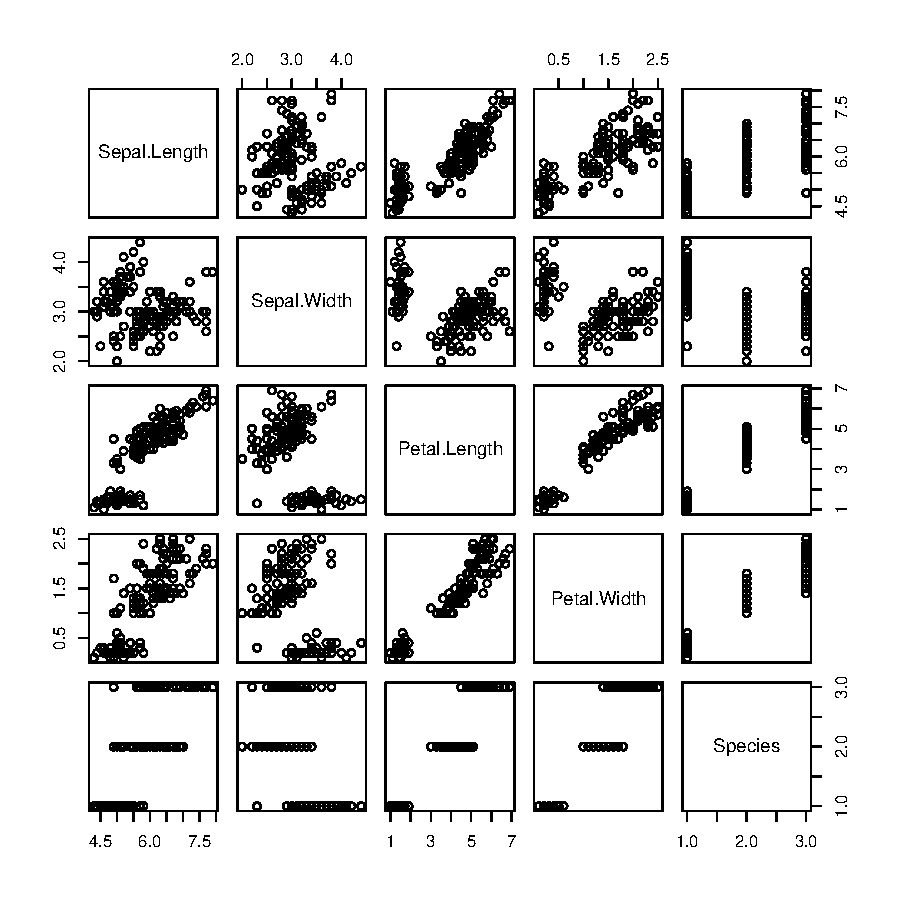
\includegraphics{Sweave-test-1-006}
\end{center}
\caption{Pairs plot of the iris data.}
\end{figure}

\begin{figure}[tbph]
\begin{center}
\begin{Sinput}
> boxplot(Sepal.Length ~ Species, data = iris)
\end{Sinput}
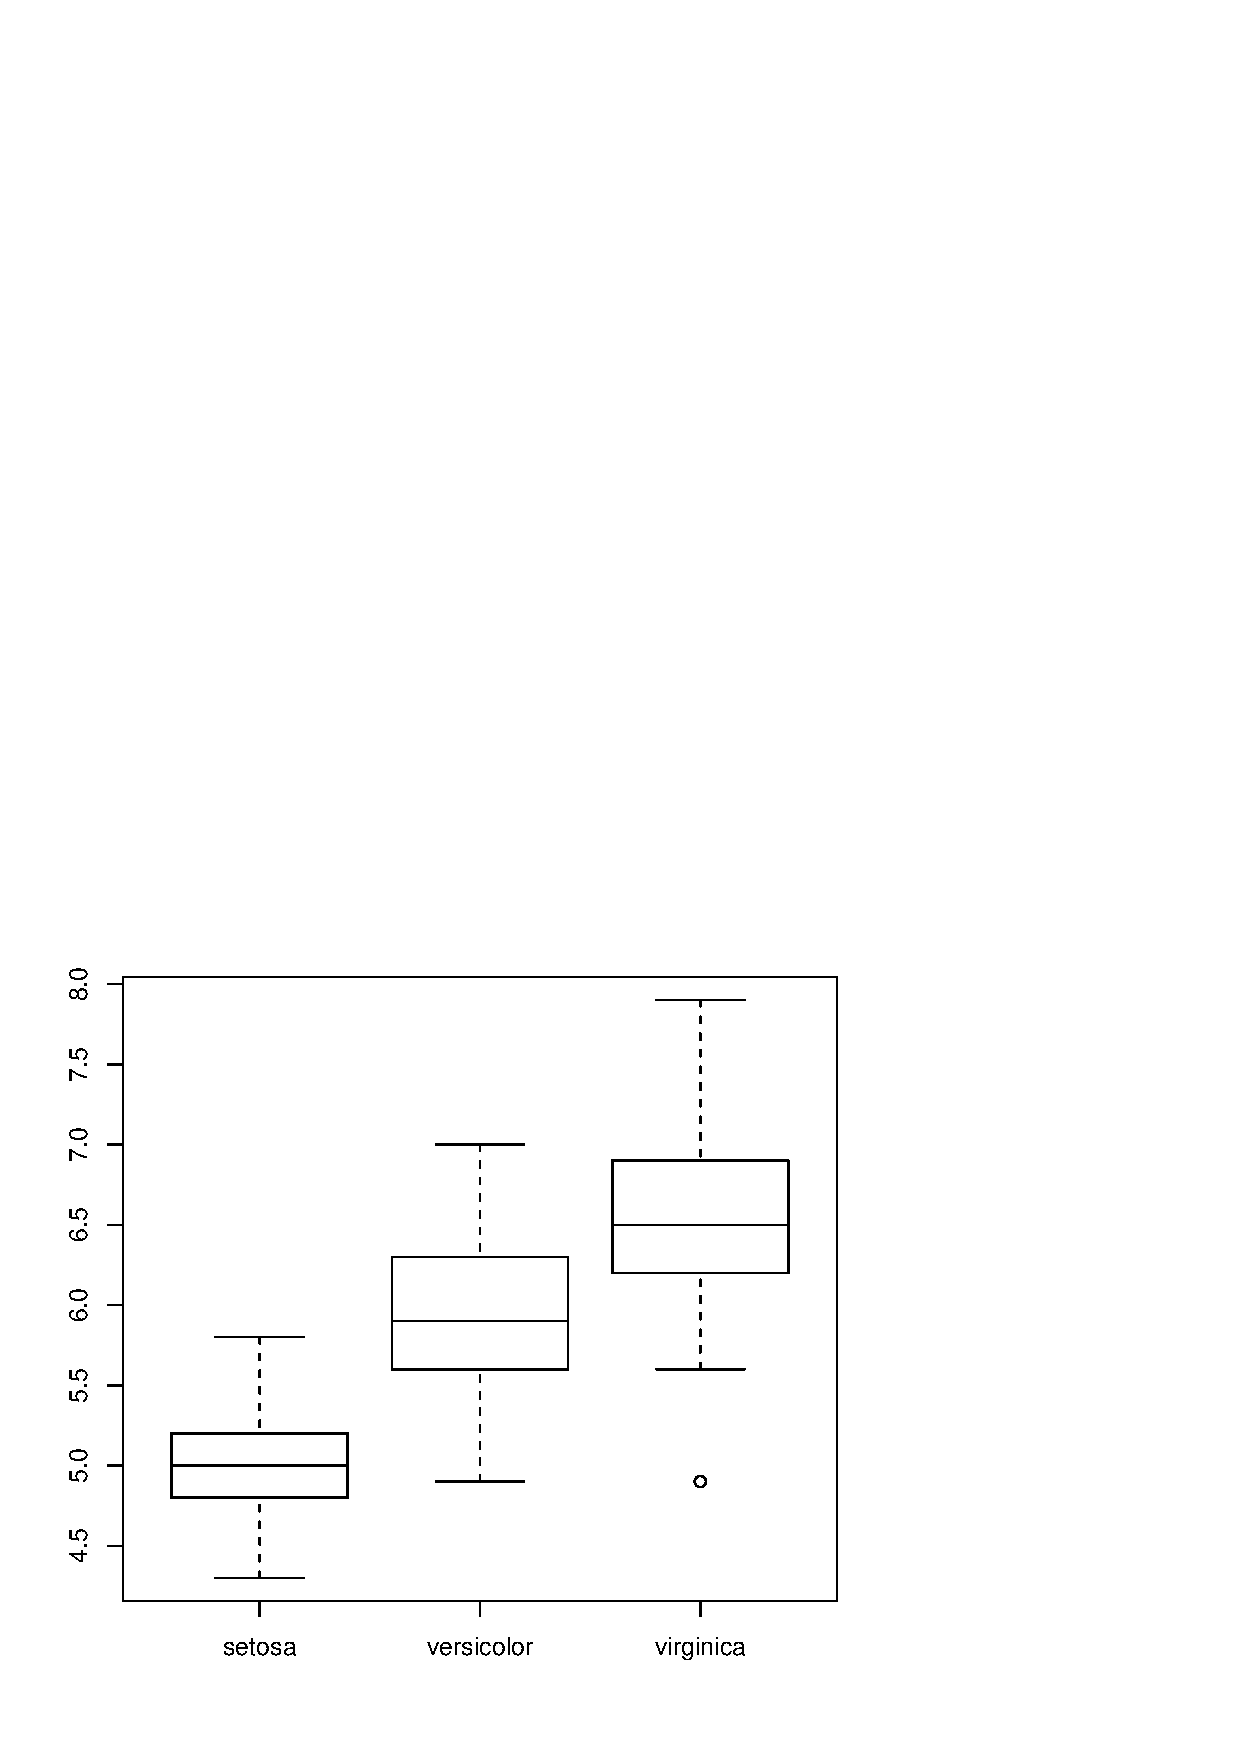
\includegraphics{Sweave-test-1-007}
\end{center}
\caption{Boxplot of sepal length grouped by species.}
\end{figure}

% R is not Splus, hence this chunk will be ignored:

\end{document}
